\subsection{Simulation}
\begin{figure}[h]
	\centering
	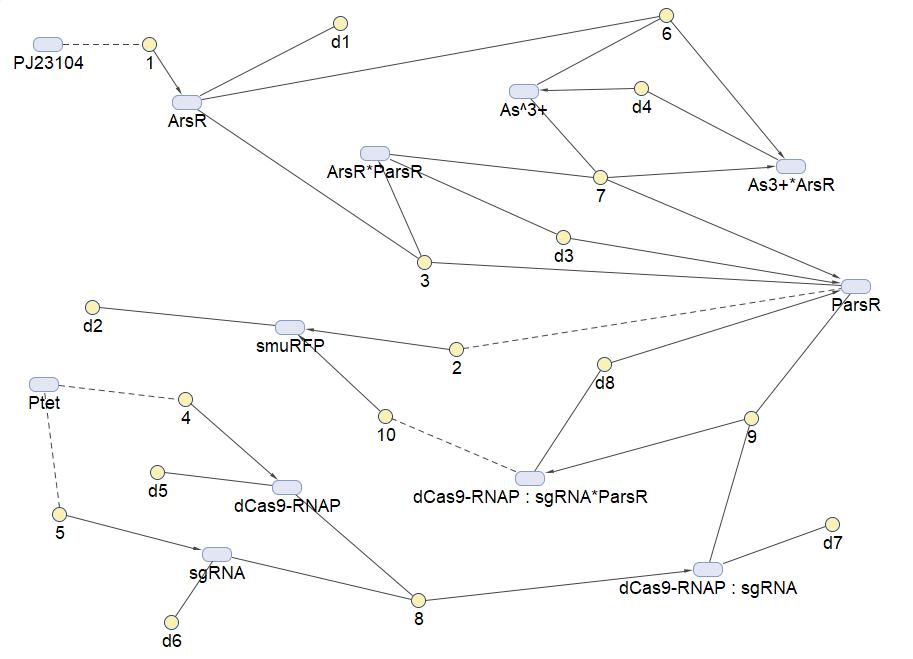
\includegraphics[width=10cm,height=7cm]{screenshot003}	
	\caption{reaction map generated from the reaction set above using SimBiology Toolbox}
\end{figure}
SimBiology toolbox provides functions for modeling, simulating, and analyzing biochemical pathways on basis of the powerful computing engine of Matlab.

\begin{figure}[h]
	\centering
	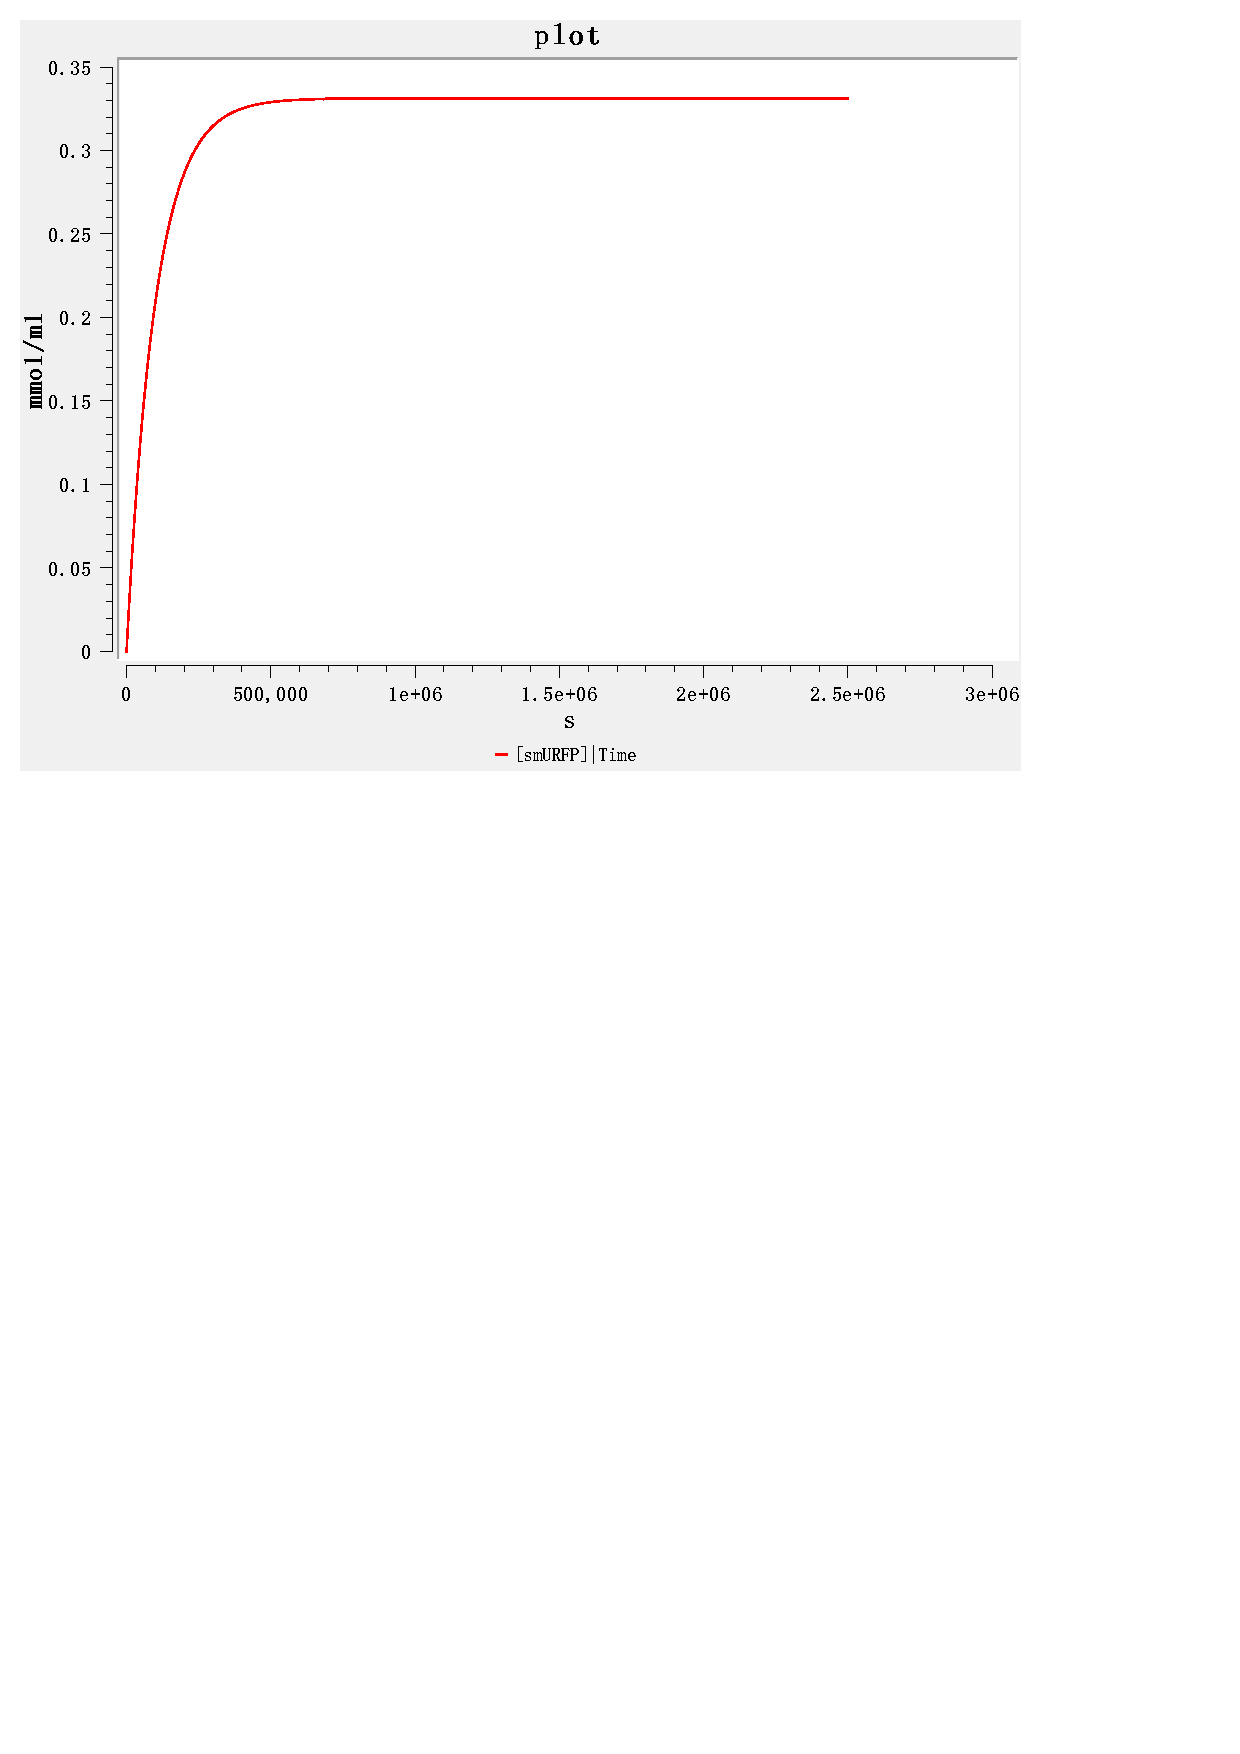
\includegraphics[width=10cm,height=10cm]{smuRFP}
	\caption{Schematic diagram of smURFP fluorescence by COPASI}
\end{figure}

COPASI is freeware developed withcollaboration of VBI and EMLR. It provides
almost the same functions as SimBiology, though not quite powerful. But compared with SimBiology, it provides a friendly user interface for model analysis, such as parameter estimation,and parameter scan.

Through the figure, we can see that the smURFP fluorescence gradually increased and then reached a steady state after a period of time  in the presence of arsenic ions.


\subsection{Sensitivity Analysis}
A good biosystem should be with a stability towards fluctuations in parameters. And  a  good model should also reflect this and hence a test for robustness can be an important test of the model.
Robustness analysis can also pinpoint which reactions/parameters that are important for obtaining a specific biological behavior. A simple measure for sensitivity is to measure the relative change of a system feature due to a change in a parameter. As for our model, the feature can be the equilibrium concentration of the smuRFP,C for which the sensitivity (S) to a parameter k is:
\begin{equation}
S=\frac{\frac{dC}{C}}{\frac{dk}{k}}=\frac{dC}{dk}\frac{k}{c}\approx \frac{\Delta C}{\Delta k}\frac{k}{c}
\end{equation}
The Matlab scripts used for sensitivity analysis see attached.
\begin{figure}
	\centering
	\begin{varwidth}[t]{\textwidth}
		\vspace{0pt}
		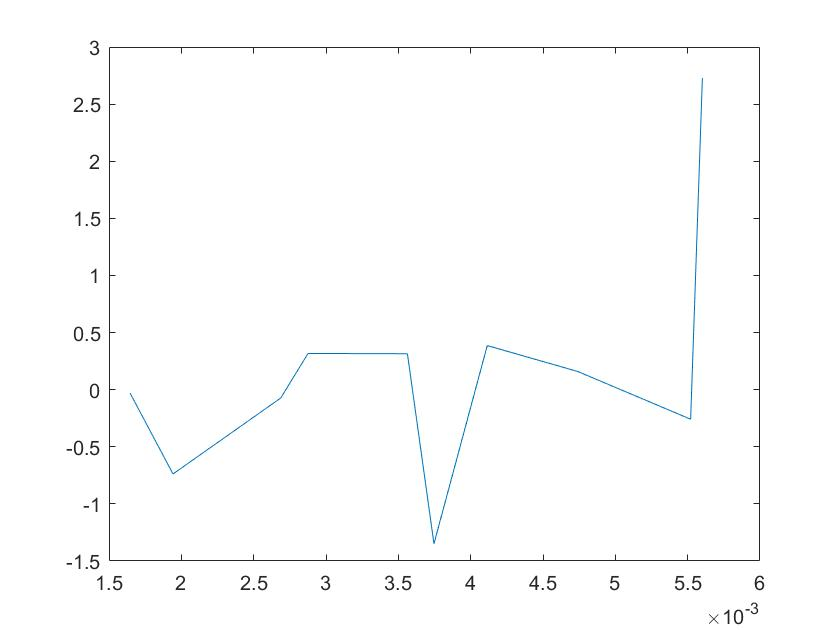
\includegraphics[height=4cm]{s1.jpg}
	\end{varwidth}%
	\caption{sensitivity of k1}
	%\qquad 
	\begin{varwidth}[t]{\textwidth}
		\vspace{0pt}
		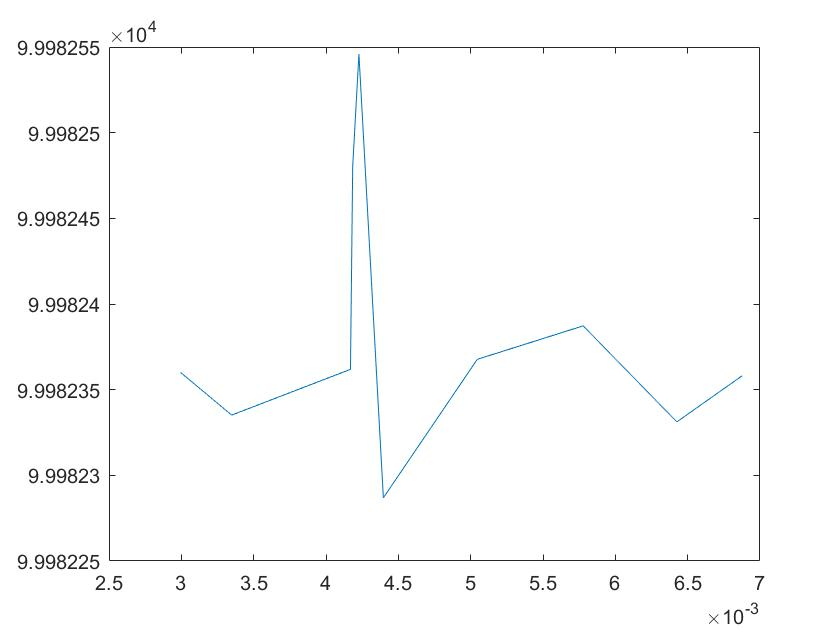
\includegraphics[height=4cm]{s2.jpg}
	\end{varwidth}
	\caption{sensitivity of k2}
	\begin{varwidth}[t]{\textwidth}
		\vspace{0pt}
		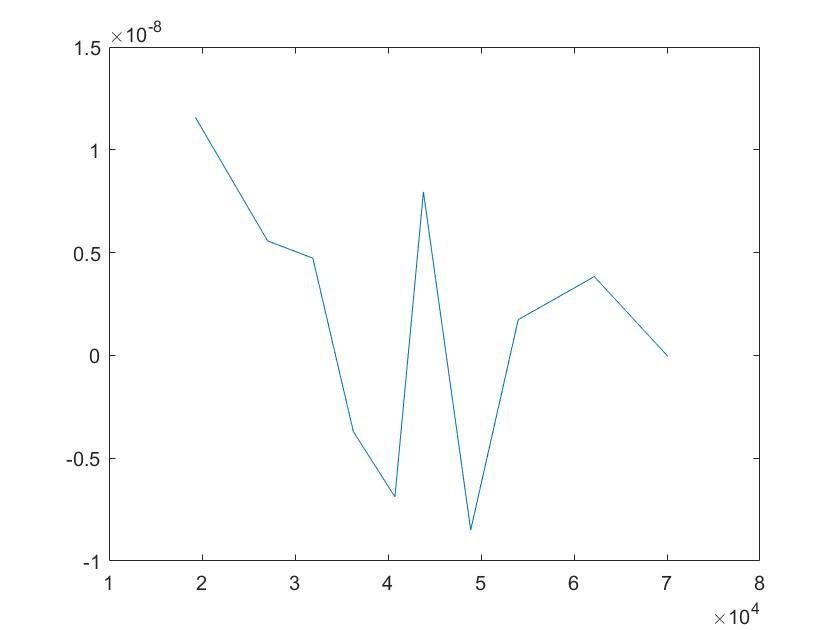
\includegraphics[height=4cm]{s3.jpg}
	\end{varwidth}
	\caption{sensitivity of k3}
	\begin{varwidth}[t]{\textwidth}
		\vspace{0pt}
		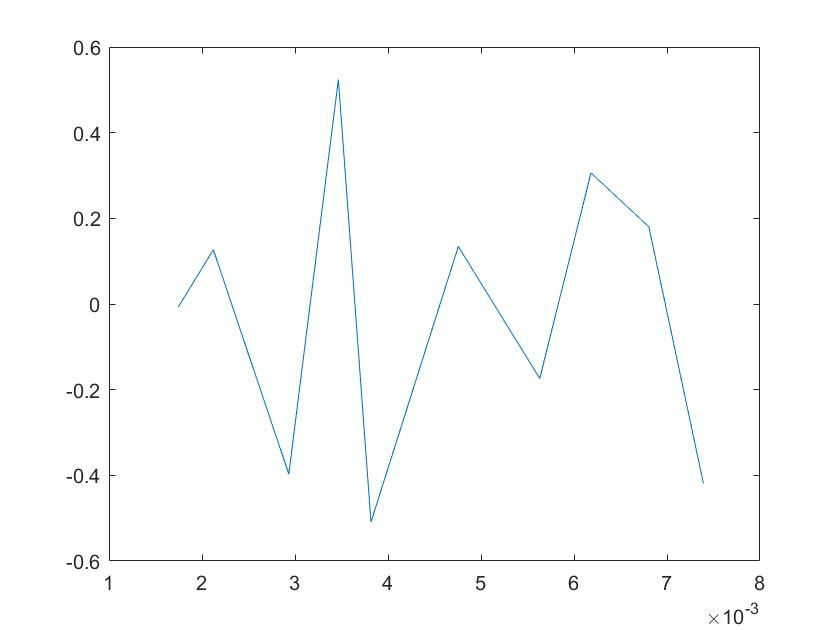
\includegraphics[height=4cm]{s4.jpg}
	\end{varwidth}
	\caption{sensitivity of k4}
	\begin{varwidth}[t]{\textwidth}
		\vspace{0pt}
		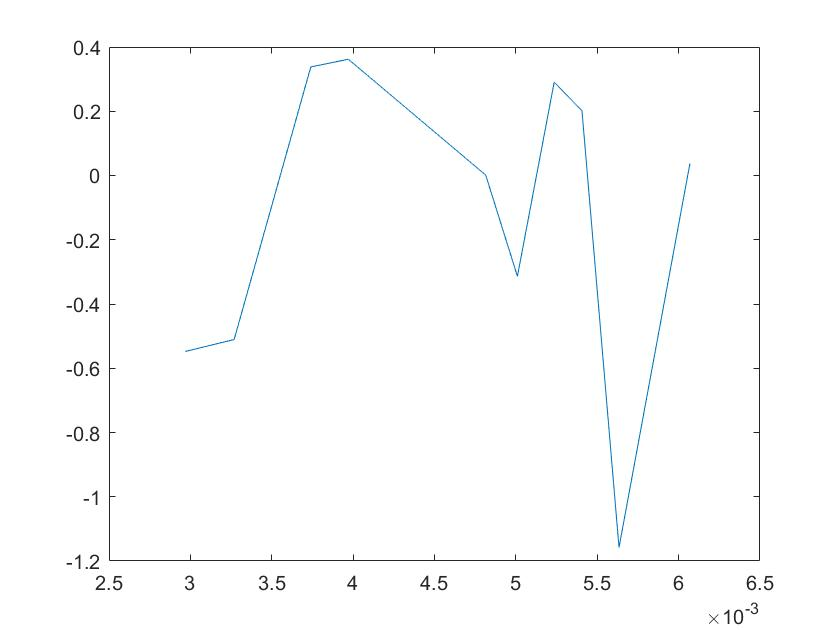
\includegraphics[height=4cm]{s5.jpg}
	\end{varwidth}
	\caption{sensitivity of k5}
	\begin{varwidth}[t]{\textwidth}
		\vspace{0pt}
		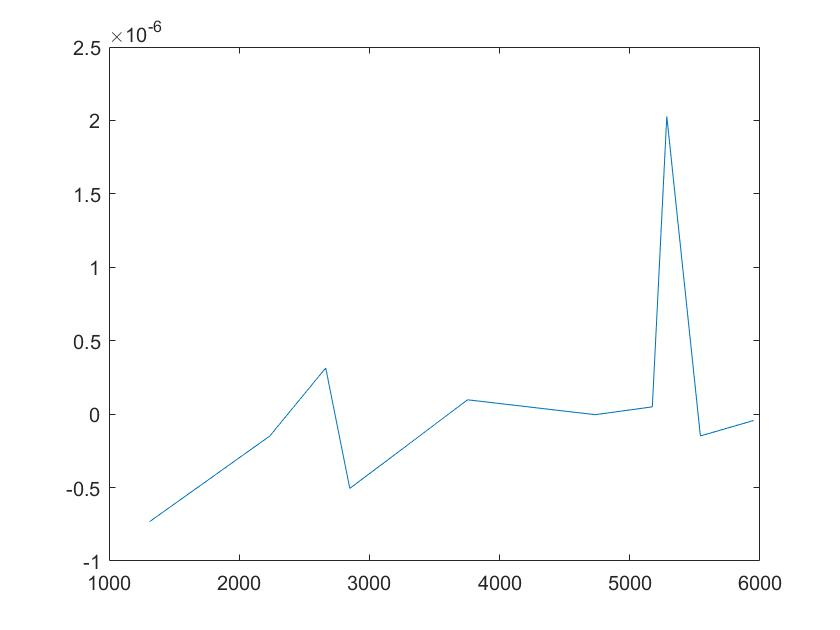
\includegraphics[height=4cm]{s6.jpg}
	\end{varwidth}
	\caption{sensitivity of k6}
	\begin{varwidth}[t]{\textwidth}
		\vspace{0pt}
		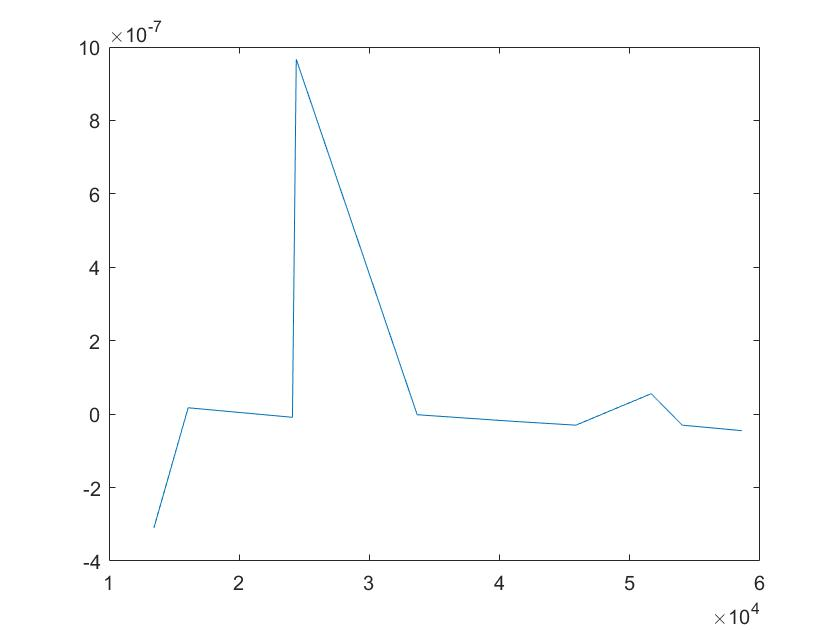
\includegraphics[height=4cm]{s7.jpg}
	\end{varwidth}
	\caption{sensitivity of k7}
	\begin{varwidth}[t]{\textwidth}
		\vspace{0pt}
		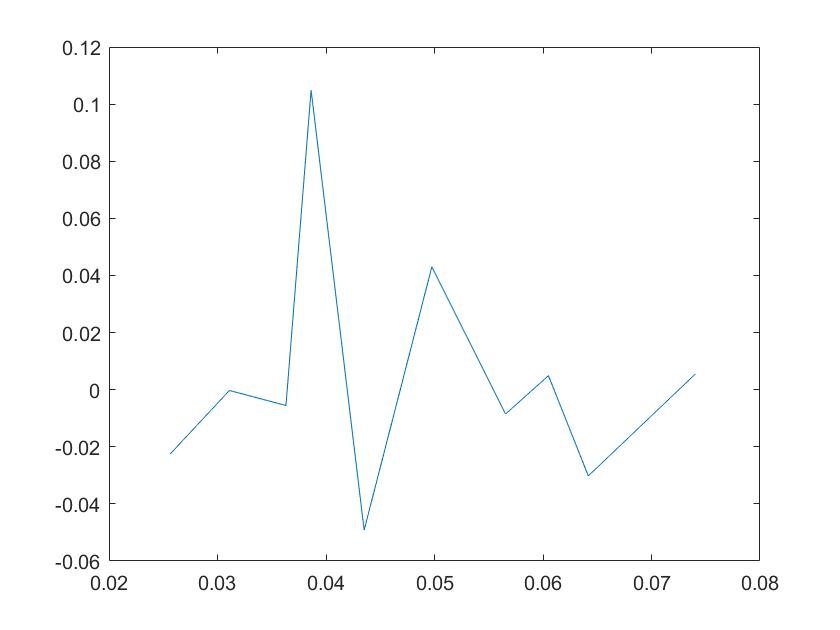
\includegraphics[height=4cm]{s8.jpg}
	\end{varwidth}
	\caption{sensitivity of k8}
	\begin{varwidth}[t]{\textwidth}
		\vspace{0pt}
		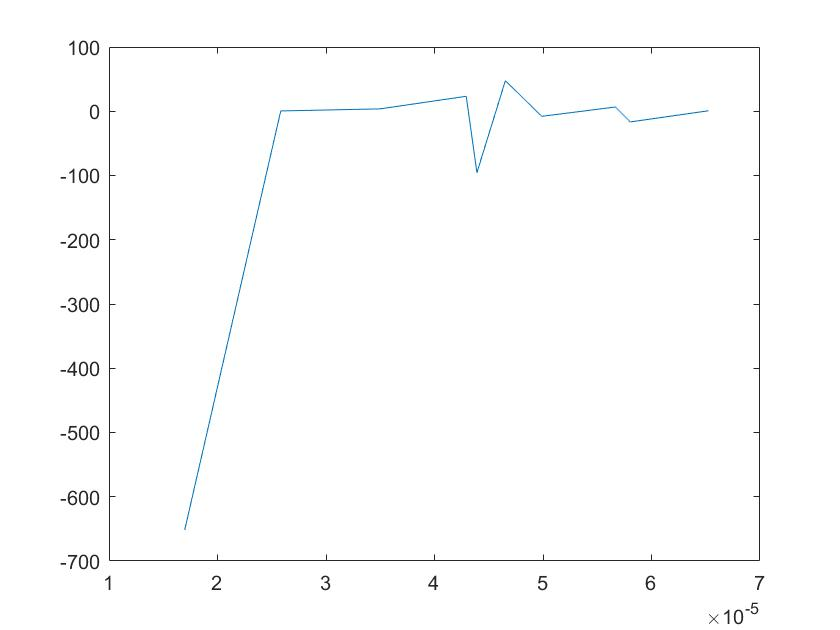
\includegraphics[height=4cm]{s9.jpg}
	\end{varwidth}
	\caption{sensitivity of k9}
	\begin{varwidth}[t]{\textwidth}
		\vspace{0pt}
		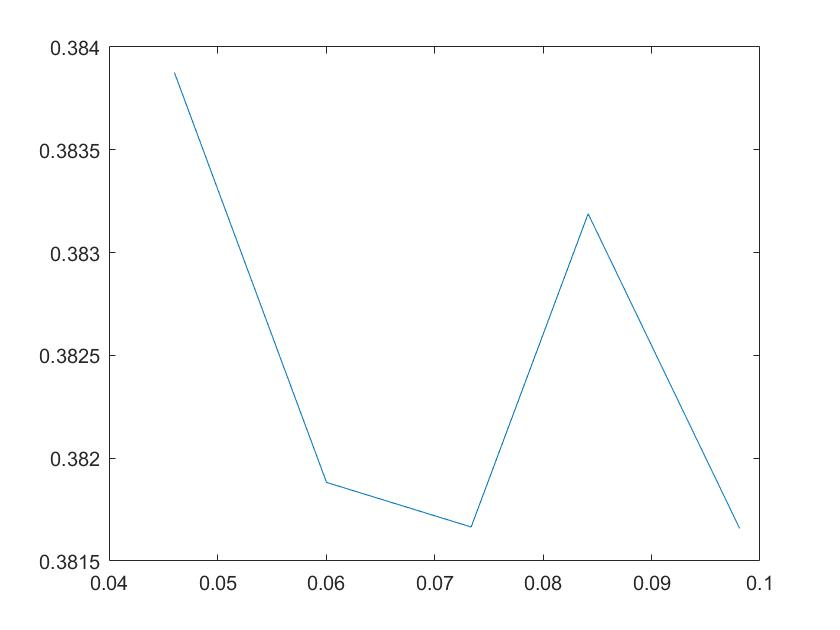
\includegraphics[height=4cm]{s10.jpg}
	\end{varwidth}
	\caption{sensitivity of k10}
	\begin{varwidth}[t]{\textwidth}
		\vspace{0pt}
		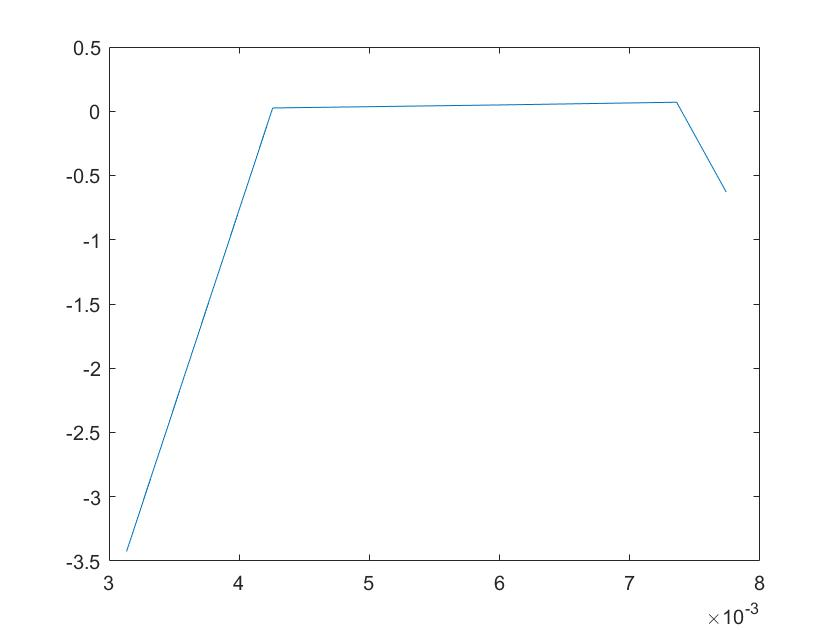
\includegraphics[height=4cm]{sd1.jpg}
	\end{varwidth}
	\caption{sensitivity of kd1}
	\begin{varwidth}[t]{\textwidth}
		\vspace{0pt}
		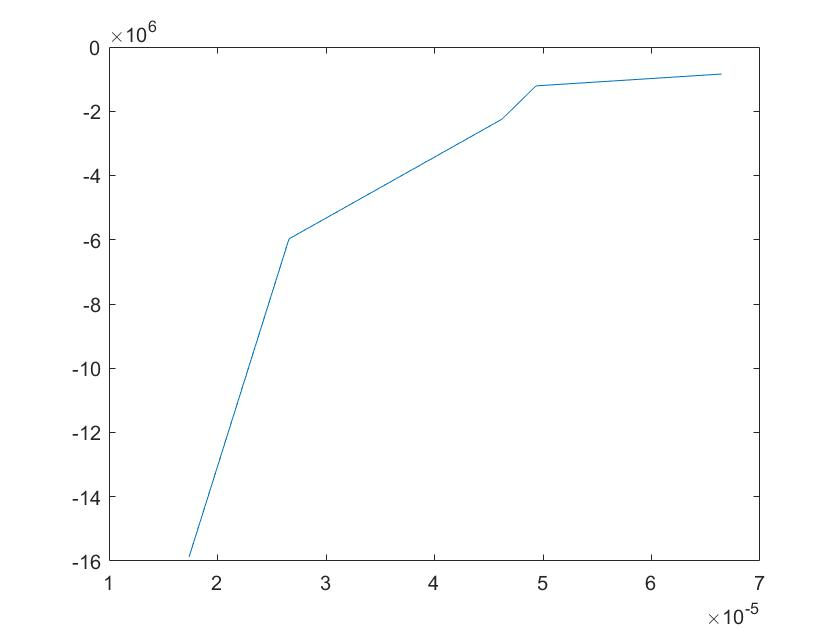
\includegraphics[height=4cm]{sd2.jpg}
	\end{varwidth}
	\caption{sensitivity of kd2}
	\begin{varwidth}[t]{\textwidth}
		\vspace{0pt}
		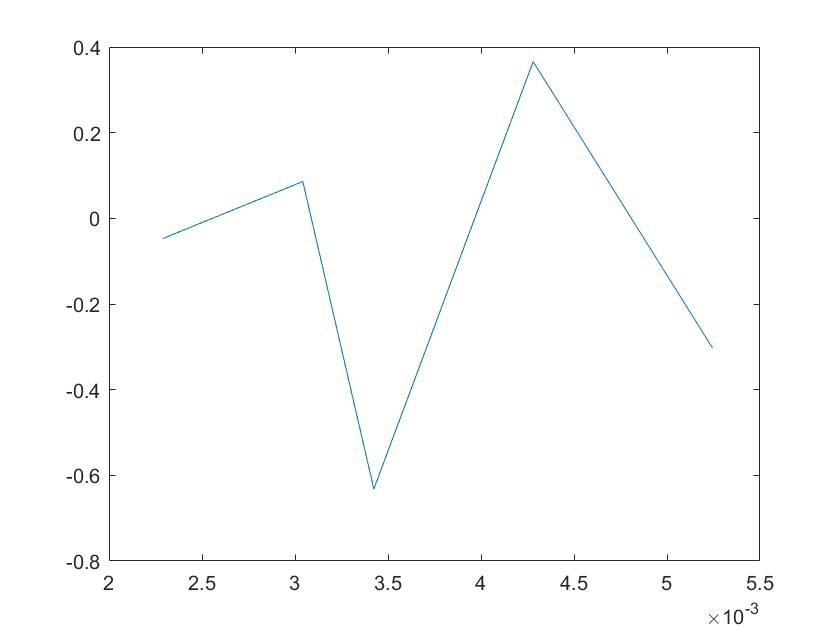
\includegraphics[height=4cm]{sd3.jpg}
	\end{varwidth}
	\caption{sensitivity of kd3}
	\begin{varwidth}[t]{\textwidth}
		\vspace{0pt}
		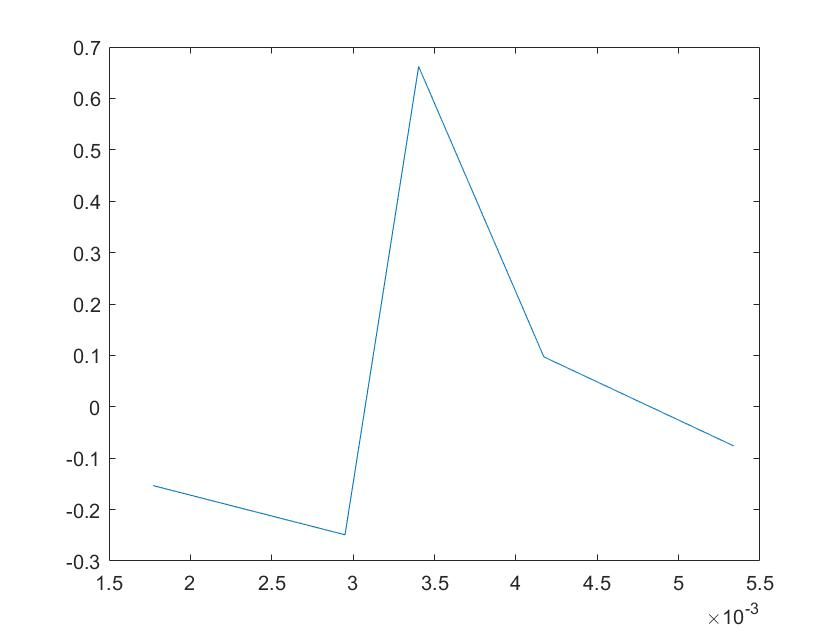
\includegraphics[height=4cm]{sd4.jpg}
	\end{varwidth}
	\caption{sensitivity of kd4}
	\begin{varwidth}[t]{\textwidth}
		\vspace{0pt}
		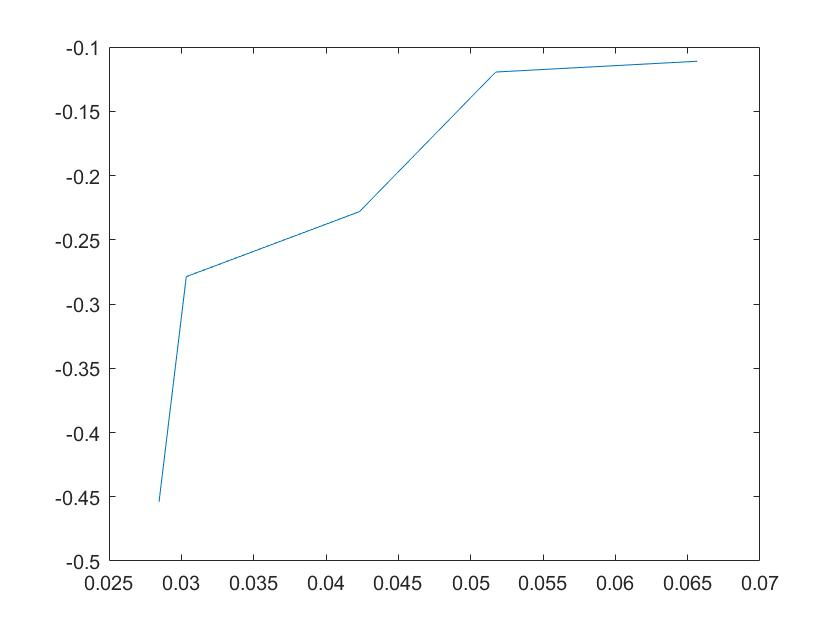
\includegraphics[height=4cm]{sd5.jpg}
	\end{varwidth}
	\caption{sensitivity of kd5}
	\begin{varwidth}[t]{\textwidth}
		\vspace{0pt}
		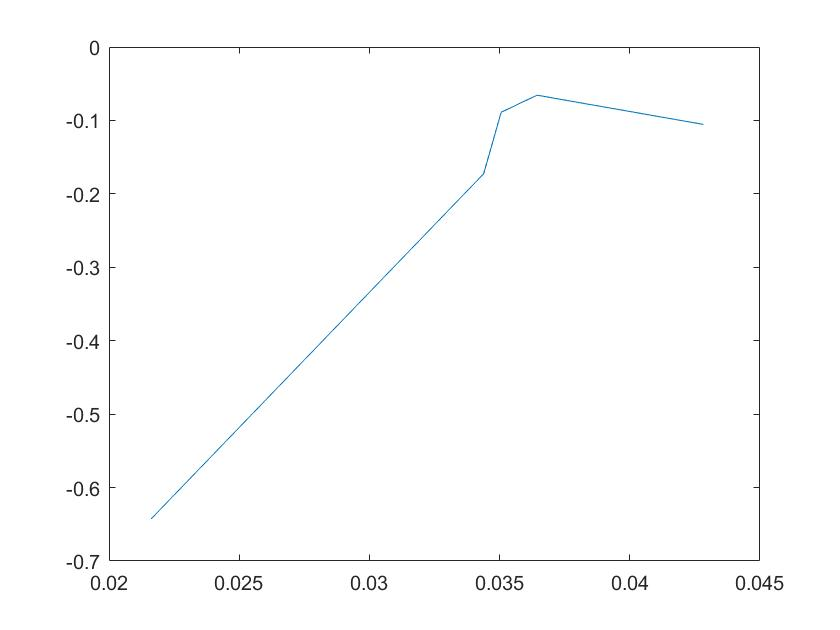
\includegraphics[height=4cm]{sd6.jpg}
	\end{varwidth}
	\caption{sensitivity of kd6}
	\begin{varwidth}[t]{\textwidth}
		\vspace{0pt}
		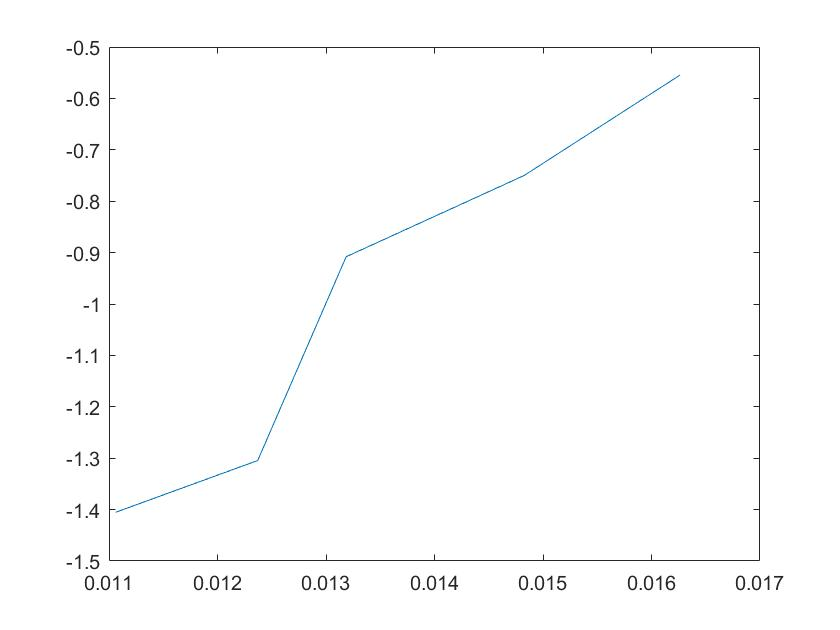
\includegraphics[height=4cm]{sd7.jpg}
	\end{varwidth}
	\caption{sensitivity of kd7}
	\begin{varwidth}[t]{\textwidth}
		\vspace{0pt}
		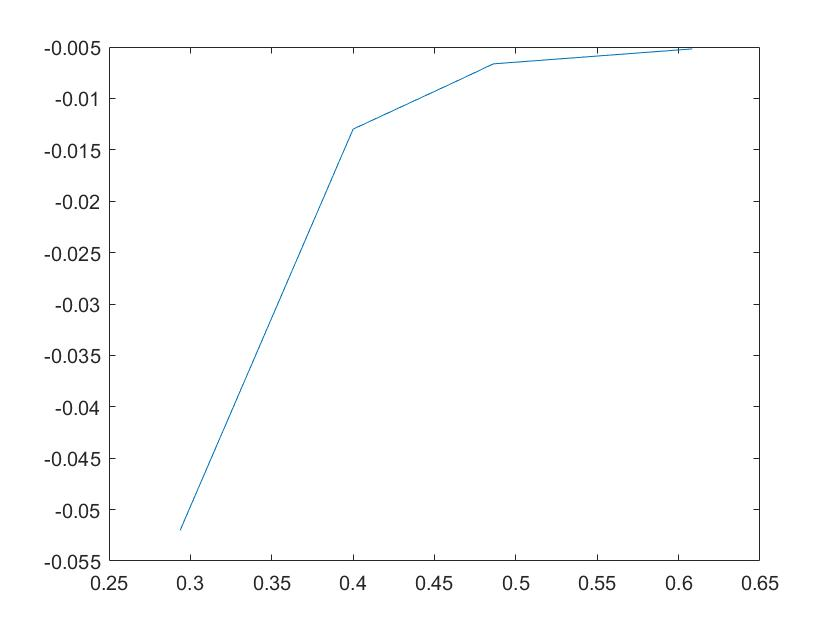
\includegraphics[height=4cm]{sd8.jpg}
	\end{varwidth}
	\caption{sensitivity of kd8}
\end{figure}

\subsection{Modification of the model}
The results are  not very satisfactory, and we suspect that it may be due to the simplification of the two processes of transcription and translation when producing proteins into a one-step process.So we take the mRNA into account, and then the reaction (1) to (4) four reactions should be replaced by the  following 6 reaction equations:
\begin{equation}
P_{J23104} \stackrel{k_{1'}}{\longrightarrow} P_{J23104}+mRNA_{ArsR}
\end{equation}
\begin{equation}
mRNA_{ArsR}\stackrel{k_{2'}}{\longrightarrow} mRNA_{ArsR}+ArsR
\end{equation}
\begin{equation}
P_{arsR} \stackrel{k_{3'}}{\longrightarrow} P_{arsR} +mRNA_{smURFP}
\end{equation}
\begin{equation}
mRNA_{smURFP} \stackrel{k_{4'}}{\longrightarrow} mRNA_{smURFP}+ smURFP
\end{equation}
\begin{equation}
P_{tet} \stackrel{k_{5'}}{\longrightarrow} P_{tet} +mRNA_{dCas9-RNAP}
\end{equation}
\begin{equation}
mRNA_{dCas9-RNAP} \stackrel{k_{6'}}{\longrightarrow} mRNA_{dCas9-RNAP}+dCas9-RNAP
\end{equation}
And the reaction equation set for the degradation of the reaction substance should also be added to the following two reaction equations.
\begin{equation}
mRNA_{ArsR}\stackrel{k_{d9}}{\longrightarrow}Ø
\end{equation}
\begin{equation}
mRNA_{smURFP}\stackrel{k_{d10}}{\longrightarrow}Ø
\end{equation}
\begin{equation}
mRNA_{dCas9-RNAP}\stackrel{k_{d11}}{\longrightarrow}Ø
\end{equation}
Added parameter values:
\begin{table}[htbp]
	\centering
	\caption{\label {tab:test} Parameters}
	\begin{tabular}{cccccccccccccccccc}
		\toprule
		Rate constants & Value& units & source \\
		\midrule
		k1' & 1.5e-2&$s^{-1} $& Berset et al. \\
		k2' & 7.33e-2 &$s^{-1} $& Berset et al.\\
		k3' & 1.5e-2 & $s^{-1}$ & Berset et al.\\
		k4' &1.84e-13&$s^{-1}$& Berset et al.\\
		k5'&  &$s^{-1}$&  \\
		k6' &    & $s^{-1}$ &   \\
		kd9&2.81e-3  & $ns^{-1}$ & Berset et al.  \\
		kd10  &7.62e-3 &$s^{-1}$ & Berset et al. \\
		kd11& & $s^{-1}$& \\
		
		\bottomrule
	\end{tabular}
\end{table}

\subsection{a bold assumption}
Since the goal of our project is to try to increase the sensitivity of biosensors by introducing a complex of dcas9-RNAP and sgRNA, and the purpose of our model is to explore whether this complex is effective. So why not assume a reasonable and large enough concentration value for this complex. We use the concentration of glyceraldehyde-3-phosphate dehydrogenase A as the assumed concentration. Glyceraldehyde 3 phosphate dehydrogenase A (gapA) is a key enzyme in the glycolytic pathway, and the gene encoding this enzyme is a housekeeping gene in E. coli cells with high expression levels. We found in the literature that the protein mass of gapA is 48645fg/cell, and its molecular weight is 35492 Da.The amount of abundance of Glyceraldehyde 3 phosphate dehydrogenase A protein per cell can be calculated as follows:

\begin{displaymath}
n=\frac{m}{M}=\frac{48645*10^{-15}g}{35492g/mol}=1.37*10^{-15}mol
\end{displaymath}
As for the size of E. coli, we found relevant data from the literature, see the figure below.

\begin{figure}[!htbp]
	\centering
	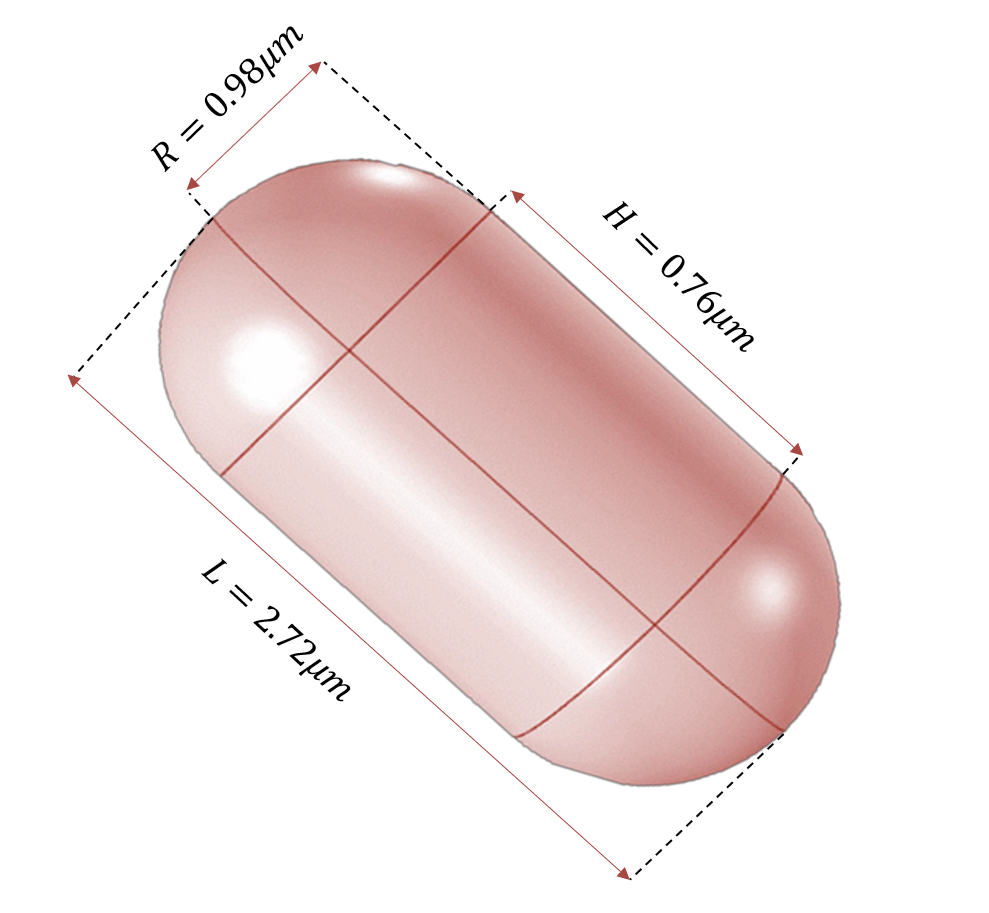
\includegraphics[width=7cm,height=7cm]{dc}
	\caption{size of E. coli}
\end{figure}

The volume of E. coli can be calculated as follows:
\begin{displaymath}
V_{E.coli}=\frac{4}{3} \pi R^3+\pi R^2H=\frac{4}{3} \pi (0.98\mu m)^3+\pi (0.98\mu m)^2(0.76\mu m)=6.24\mu m^3=6.24*10^{-15}L
\end{displaymath}

Then the concentration of Glyceraldehyde 3 phosphate dehydrogenase A protein in the cell can be determined:
\begin{displaymath}
c=\frac{n}{V_{E.coli}}=\frac{1.37*10^{-15}mol}{6.24*10^{-15}L}=0.22mol/L
\end{displaymath}
With this concentration, we got very nice results:

\begin{figure}[!htbp]
	\centering
	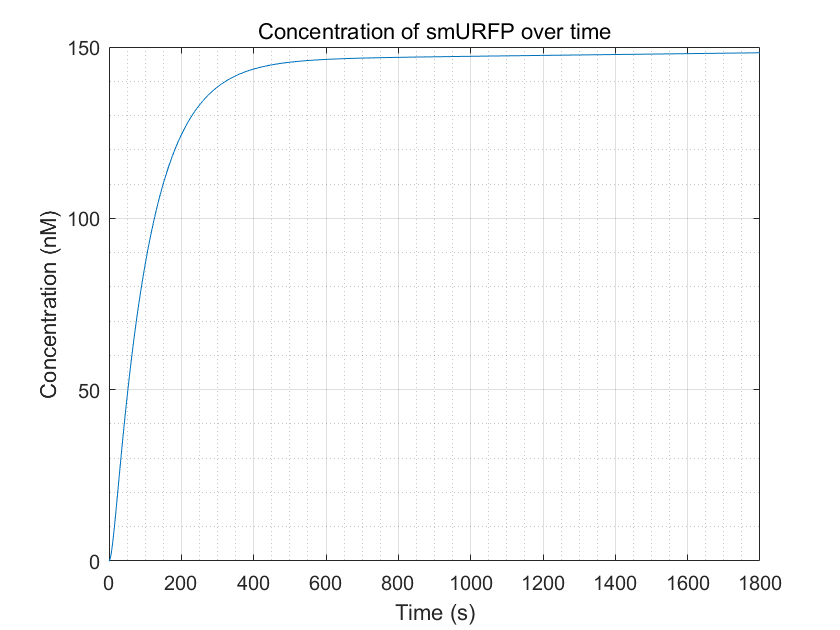
\includegraphics[width=7cm,height=7cm]{23}
	\caption{Schematic diagram of smURFP fluorescence}
\end{figure}
Compared to the diagram without introducing dcas9:
\begin{figure}[!htbp]
	\centering
	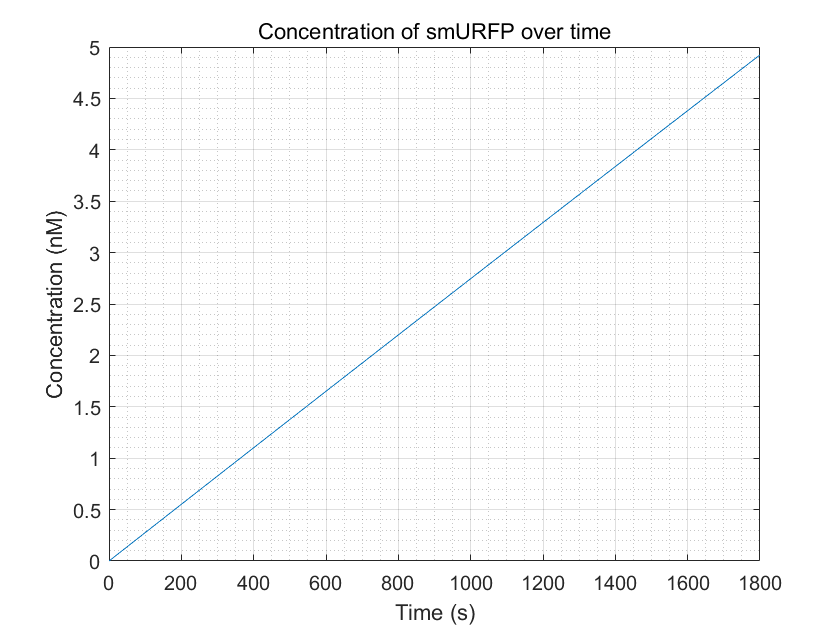
\includegraphics[width=7cm,height=7cm]{21}
	\caption{smURFP fluorescence within a reasonable time frame}
\end{figure}
\begin{figure}[!htbp]
	\centering
	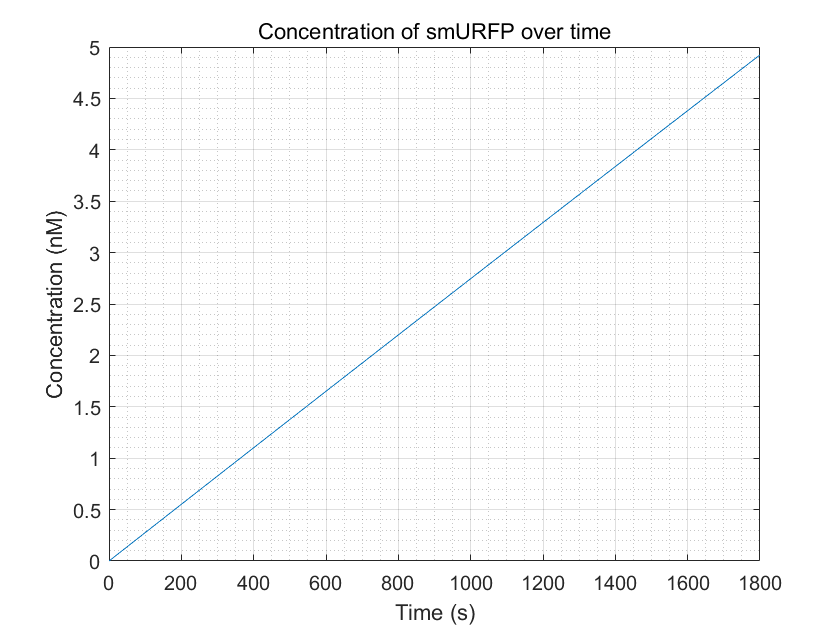
\includegraphics[width=7cm,height=7cm]{21}
	\caption{smURFP fluorescence reaches equilibrium but costs too long}
\end{figure}
From these three figures, we can conclude that dCas9-RNAP:sgRNA does have the effect of promoting transcription and increasing fluorescence intensity, thereby increasing sensitivity, as long as its concentration is sufficient. This result enhances the confidence of the experimental group, they just need to try to improve the expression of dCas9-RNAP:sgRNA in E. coli without having to doubt its role.



